%%%%%%%%%%%%%%%%%%%%%%%%%%%%%%%%%%%%%%%%%%%
%\subsection{Описание предметной области}
\subsection{Пример процесса проектирования некоторого технического устройства}
%%%%%%%%%%%%%%%%%%%%%%%%%%%%%%%%%%%%%%%%%%%
\begin{frame}%[allowframebreaks=0.9,t]

Рассмотрим процесс проектирования некоторого технического объекта на примере мобильного робота.
\begin{figure}[!ht]
  \begin{minipage}{0.455\linewidth}
    Выделим следующие компоненты:
    \begin{itemize}
      \arrowitem двигатели;
      \arrowitem пила;
      \arrowitem манипулятор;
      \arrowitem колёса;
      \arrowitem привод пилы;
      \arrowitem привод колёс;
      \arrowitem батарейный отсек;
      \arrowitem электронные компоненты;
      \arrowitem корпус;
      \arrowitem ...
    \end{itemize}
  \end{minipage}%
  \begin{minipage}{0.455\linewidth}
    \centering
    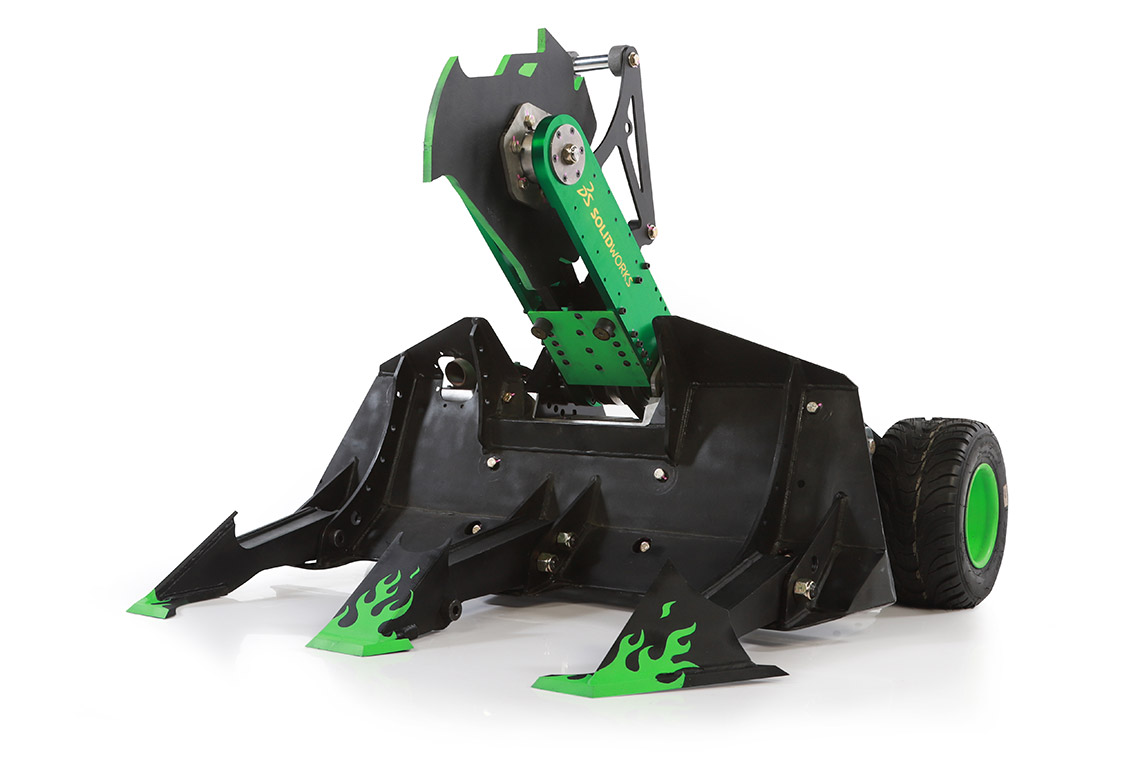
\includegraphics[width=\textwidth]{images/robot.jpg}
    \caption{Пример проектируемого объекта}
    \label{fig:technicalObjectExample}
  \end{minipage}
\end{figure}

%\onslide<1->{
%\begin{center}
%  \begin{tikzpicture}
%   \draw (0,0) -- (10,0) -- (10,3) -- (0,3) -- (0,0);
%   \end{tikzpicture}
%\end{center}}

\end{frame}
%%%%%%%%%%%%%%%%%%%%%%%%%%%%%%%%%%%%%%%%%%%
\begin{frame}[t]
	
	{\smaller[1]
	
	\onslide<1>{
	\begin{enumerate}
		\item<1-> Формулируется техническое задание.
		\item<2-> Проектируются компоненты, которые не зависят от других компонентов.
		\item<3-> Проектируются компоненты, зависящие от предыдущих.
		\item<4-> Проектируются компоненты, объединяющие или связывающие предыдущие.
		\item<5-> Проектируются компоненты, объединяющие или связывающие предыдущие.
	\end{enumerate}}
	
	
	
	
	}
	
	\begin{figure}[!ht]
    \centering
		\only<1>{%
		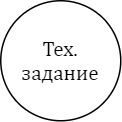
\includegraphics[scale=0.17]{images/design.frame01.png}
		}
		\only<2>{%
		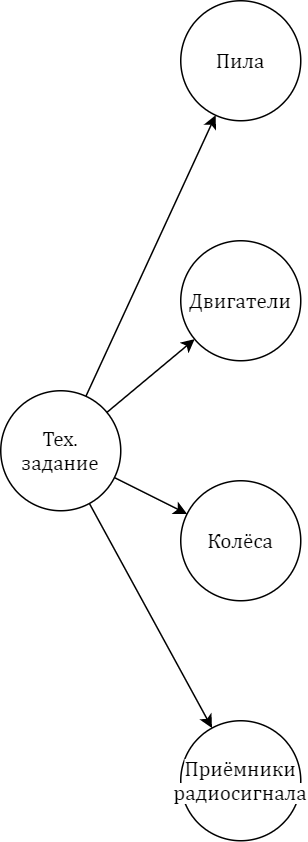
\includegraphics[scale=0.17]{images/design.frame02.png}
		}
		\only<3>{%
		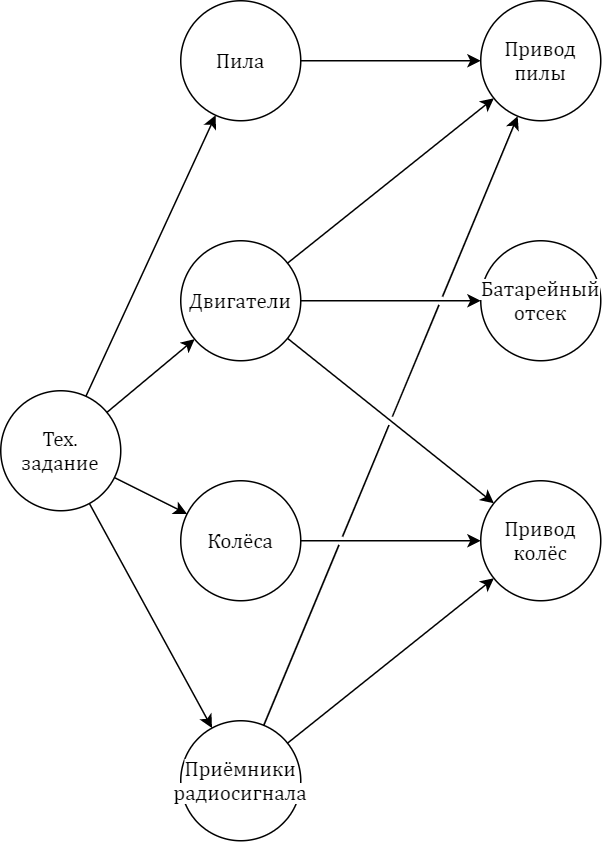
\includegraphics[scale=0.17]{images/design.frame03.png}
		}
		\only<4>{%
		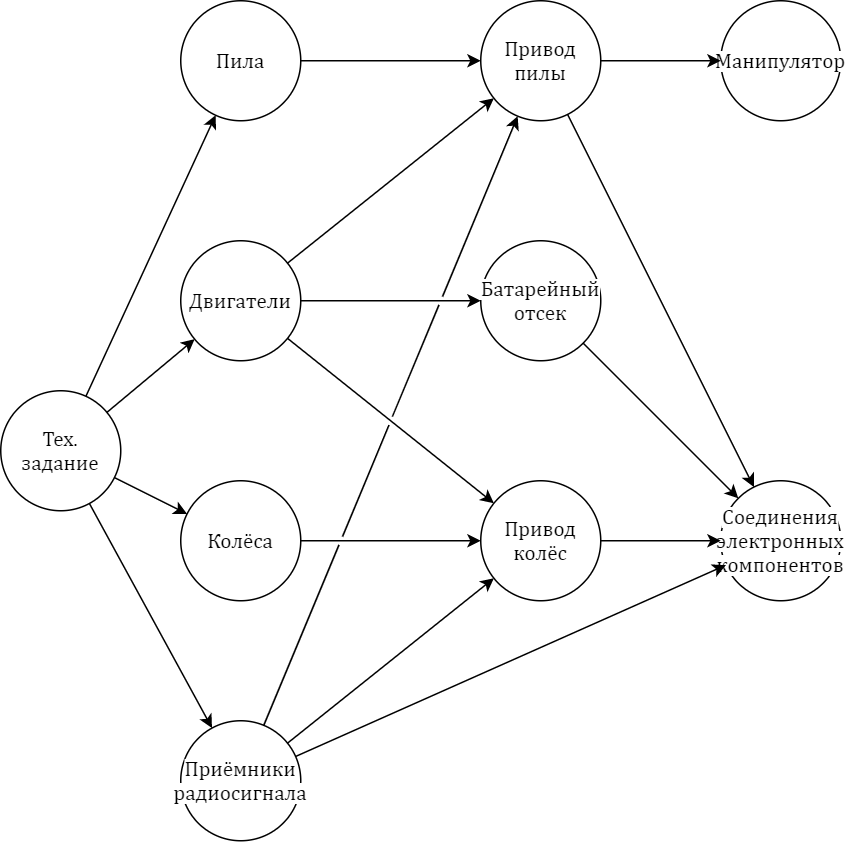
\includegraphics[scale=0.17]{images/design.frame04.png}
		}
		\only<5>{%
		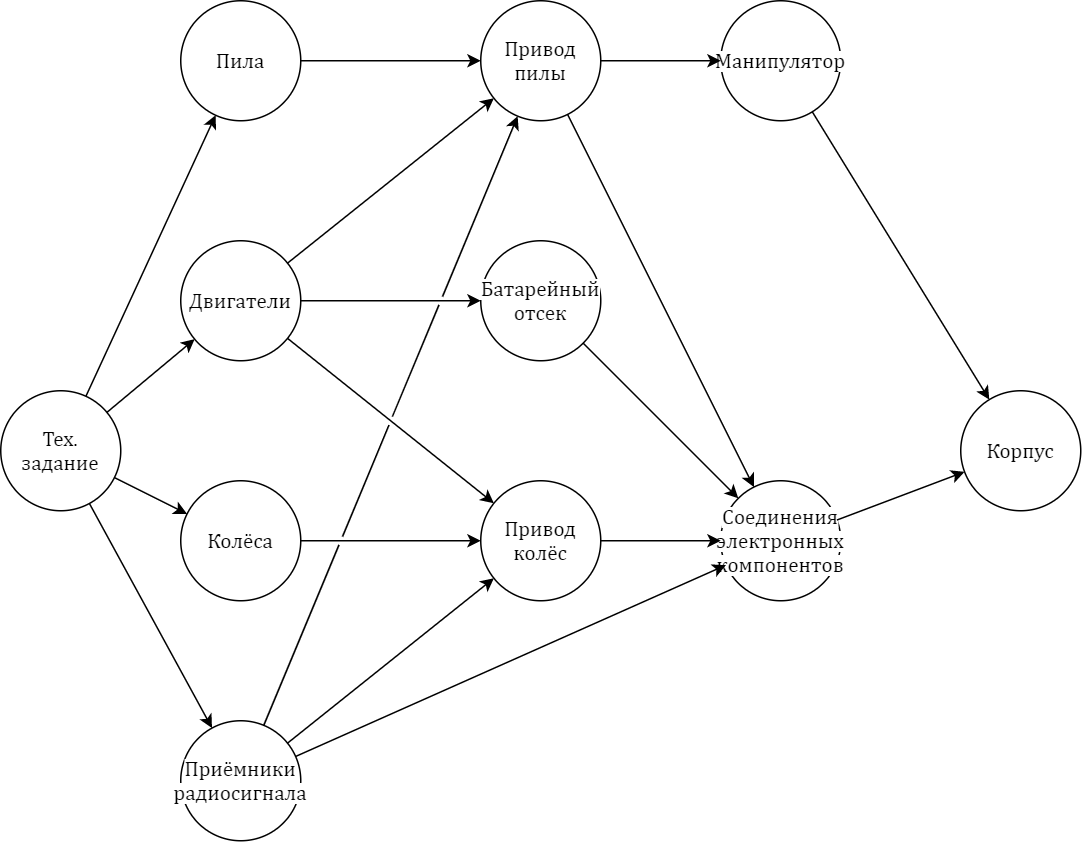
\includegraphics[scale=0.17]{images/design.frame05.png}
		}
		\caption{Проектирование мобильного робота по компонентам}\label{fig:desgin.graph}
  \end{figure}
\end{frame}


\subsection{Возможные формы представления процесса проектирования}

%%%%%%%%%%%%%%%%%%%%%%%%%%%%%%%%%%%%%%%%%%%
\begin{frame}
  \begin{remark}
    Процесс проектирования некоторого технического объекта удобно представлять в виде графа.
  \end{remark}
  \begin{figure}[!ht]
    \centering
    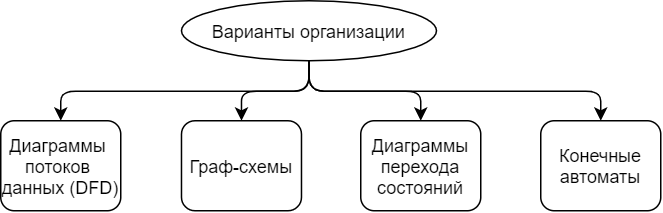
\includegraphics[width=\textwidth]{images/design_graph_variants.png}
    \caption{Различные формы организации процессов проектирования в виде графа}
    \label{fig:designGraphVariants}
  \end{figure}
\end{frame}
%%%%%%%%%%%%%%%%%%%%%%%%%%%%%%%%%%%%%%%%%%%
\subsection{Методология графоориентированного подхода (GBSE)}
%%%%%%%%%%%%%%%%%%%%%%%%%%%%%%%%%%%%%%%%%%%
\begin{frame}
  \textbf{[Идея]} Узлы графа -- состояния данных, рёбра -- переходы между ними (\emph{морфизмы}).

  \begin{figure}
    \centering
    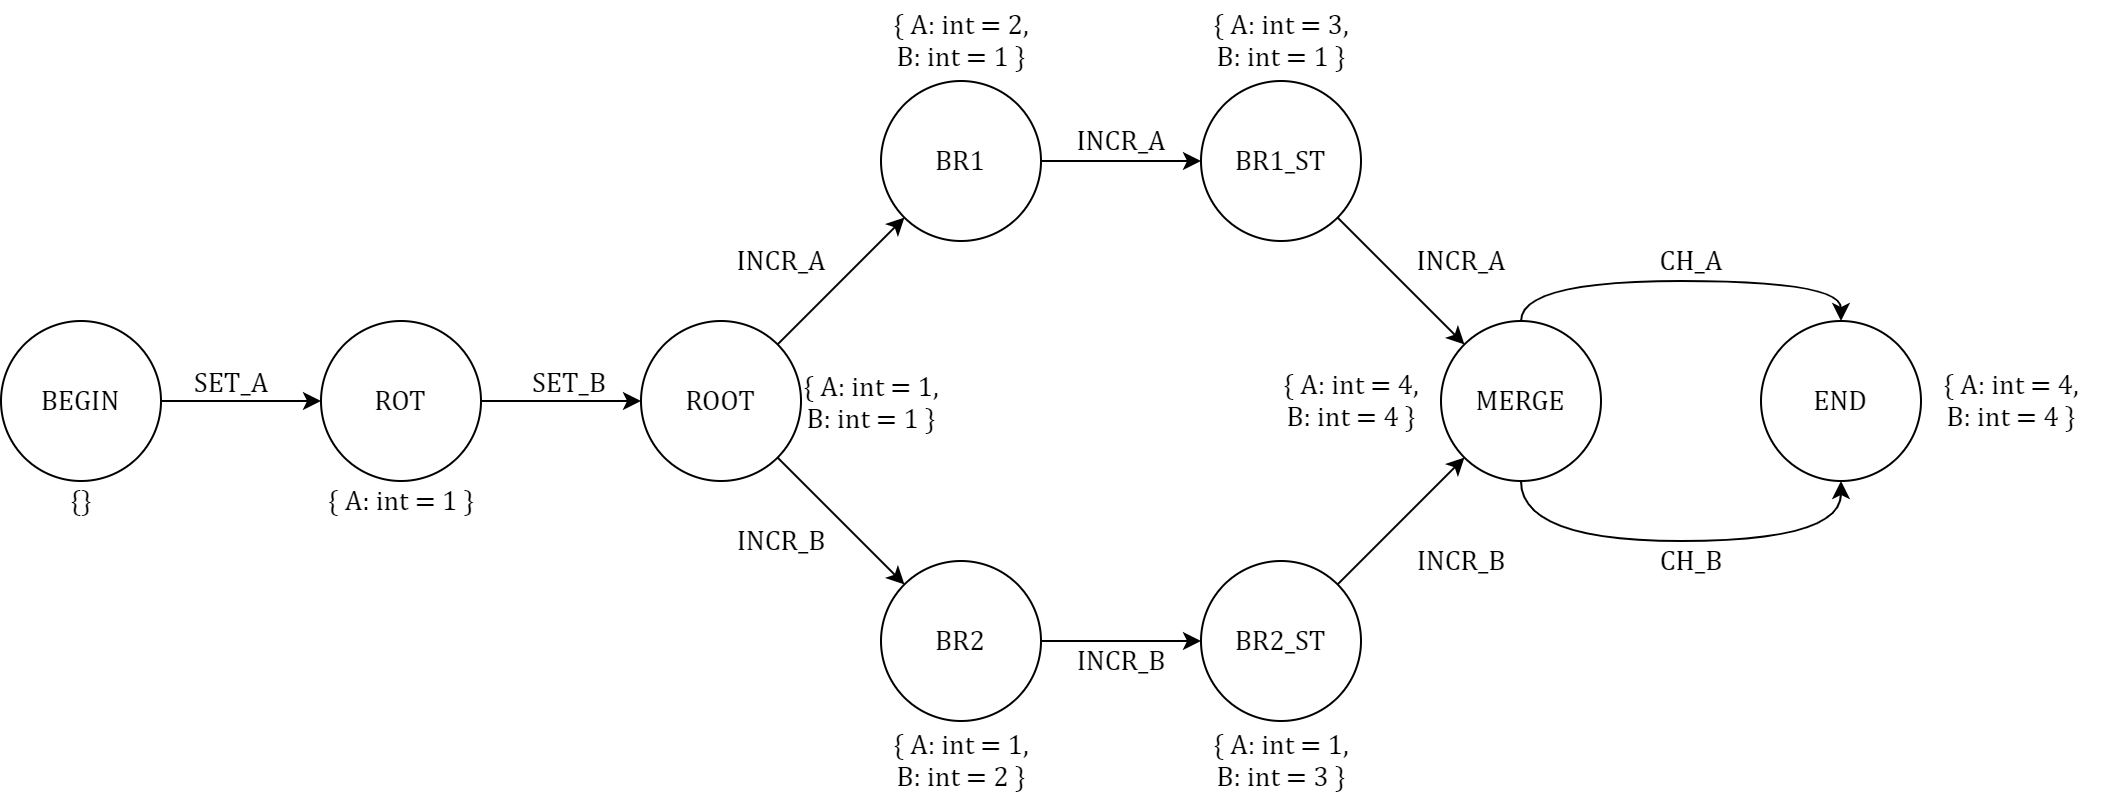
\includegraphics[width=\textwidth]{images/adot_example.png}
    \caption{Пример графовой модели вычислительного процесса}\label{fig:aDotExamplePic}
  \end{figure}
\end{frame}

\begin{frame}
%  Дополнительные определения:
  \begin{designation}
    \emph{Функция-обработчик} -- функция, обеспечивающая преобразование данных из одного состояния в другое.    
  \end{designation}
  \begin{designation}
    \emph{Функция-предикат} -- функция, определяющая соответствие подаваемого ей на вход набора данных тому виду, который требуется для выполнения отображения.
  \end{designation}
  \begin{designation}
    \emph{Функция-селектор} -- функция, отвечающая в процессе обхода графовой модели за выбор тех рёбер, которые необходимо выполнить на следующем шаге в соответствии с некоторым условием.    
  \end{designation}
\end{frame}